\chapter{项目概述}

RUCM是一种结构化和模板化的需求规格,引入了流程、结构化句型和流程控制机制。本项目以RUCM编辑器产生的rucm文件作为输入,依据课堂所讲授的RUCM规范指定相应的规则,并按照规则来自动检查一个具体的需求违反了哪些规则,同时能够支持规则的设置。


关于RUCM模型的具体介绍请参见附录\ref{appendix-2}部分领域分析报告。

\section{软件设计架构}
\begin{figure}[htbp]
    \begin{center}
        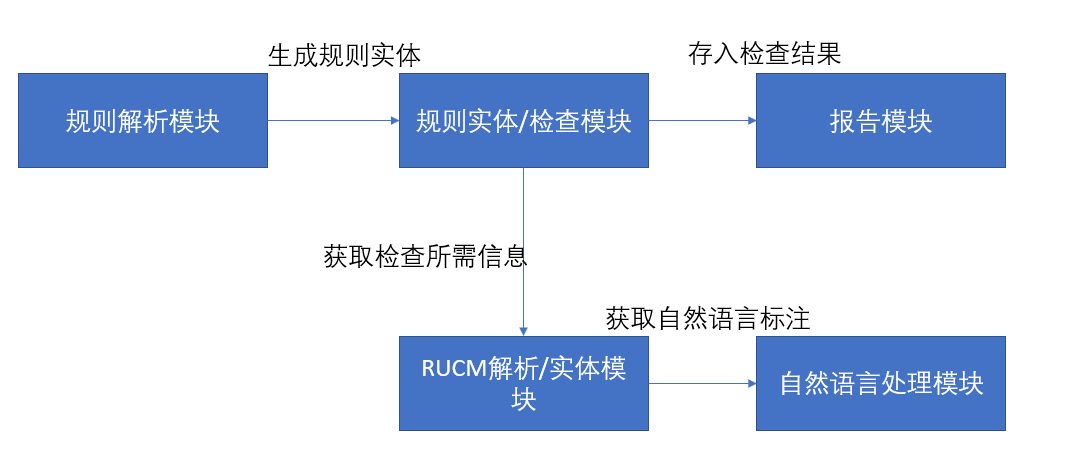
\includegraphics[scale=0.55]{src/introduction-1.png}
        \caption{软件设计架构图}
        \label{fig-introduction-1}
    \end{center}
\end{figure}

如图\ref{fig-introduction-1}所示,本软件由规则解析模块,规则实体/检查模块,报告模块,RUCM接卸/实体模块,自然语言处理模块5部分组成。

其中\textbf{规则解析模块}负责规则格式解析域检查,规则存储等功能;\textbf{规则实体/检查模块}由ComplexRule, SimpleRule, DefaultRuleXXX等部分组成,该模块的主要功能是规则的表征与检查;\textbf{规则报告模块}负责存储报告信息以及生成报;\textbf{RUCM解析/实体模块}负责检查/解析RUCM的json文件,并且将相应字段存入相应实体中并且提供对step/sentence等信息的统一查询接口;\textbf{自然语言处理模块}负责句子与词的内容分析以及相应标注。

\section{软件输入输出样例}
本软件以RUCM设计模型为输入,给出其是否符合RUCM规则的检查报告。
\subsection{输入样例}
\begin{figure}[htbp]
    \begin{center}
        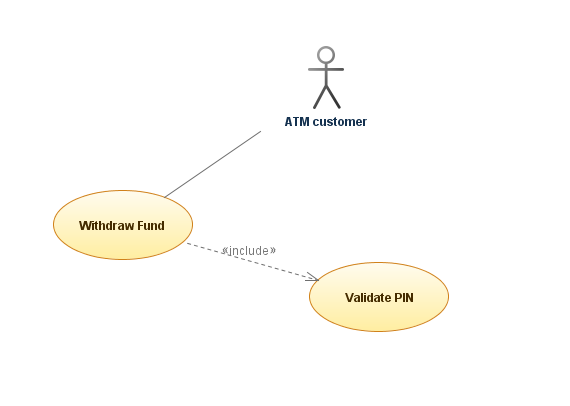
\includegraphics[scale=1.2]{src/introduction-2.png}
        \caption{用例图样例}
        \label{fig-introduction-2}
    \end{center}
\end{figure}


针对图\ref{fig-introduction-2}所示的用例图,我们写出了其用例描述\ref{fig-introduction-3},其中红线标注部分明显违背了RUCM的第5、第10两条规则,即只能使用现在时的时态(R5)与不能使用情态动词(R10)。

关于RUCM规则的具体解释请参见附录\ref{appendix-3}部分RUCM-Manual提供的官方解释。

\begin{figure}[ht]
    \begin{center}
        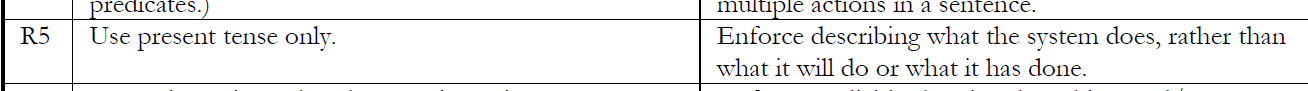
\includegraphics[scale=0.35]{src/introduction-r5.png}
        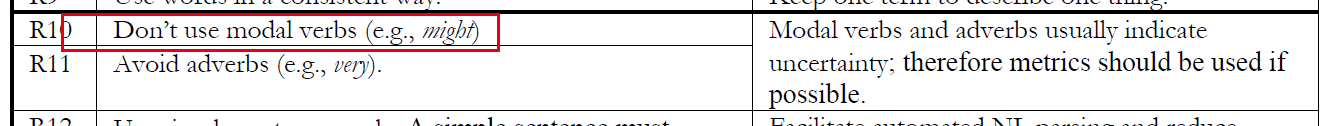
\includegraphics[scale=0.35]{src/introduction-r10.png}
        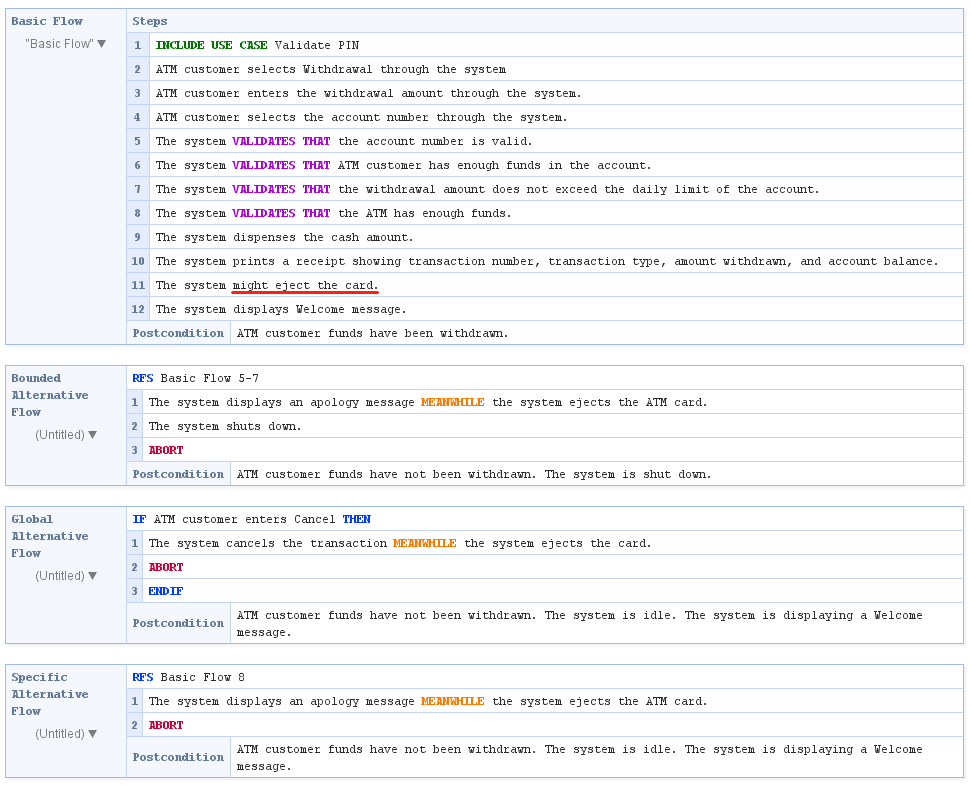
\includegraphics[scale=0.6]{src/introduction-3.png}
        \caption{RUCM样例}
        \label{fig-introduction-3}
    \end{center}
\end{figure}
\subsection{输出样例}
如图\ref{fig-introduction-4}所示,我们的软件检测到了相应的问题并输出了正确的报告。
\begin{figure}[h]
    \begin{center}
        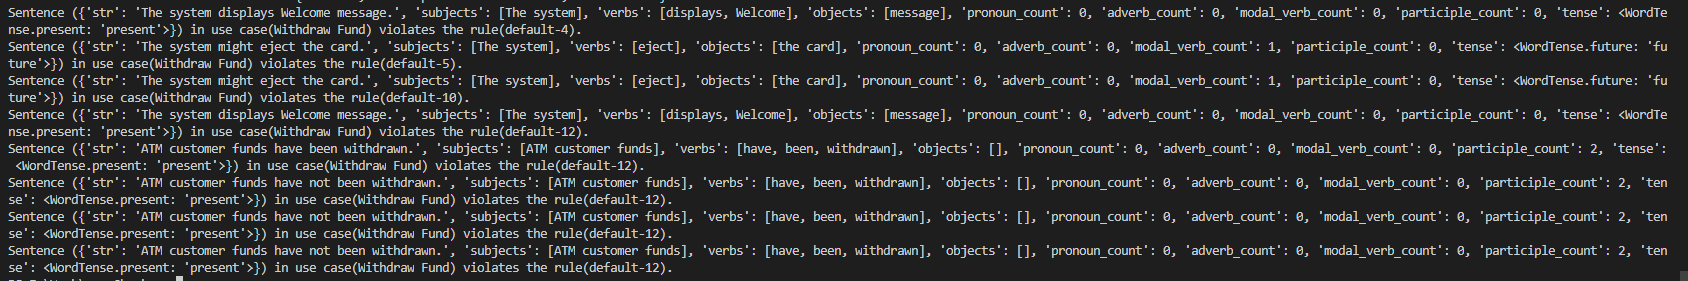
\includegraphics[scale=0.35]{src/introduction-4.png}
        \caption{命令行形式下的软件输出样例图}
        \label{fig-introduction-4}
    \end{center}
\end{figure}